
\documentclass[12pt,a4paper]{article}
\usepackage{calc}% http://ctan.org/pkg/calc
\usepackage[
  letterpaper,%
  textheight={47\baselineskip+\topskip},%
  textwidth={\paperwidth-126pt},%
  footskip=75pt,%
  marginparwidth=0pt,%
  top={\topskip+0.75in}]{geometry}% http://ctan.org/pkg/geometry
\usepackage{fancyhdr}% http://ctan.org/pkg/fancyhdr

\usepackage{graphicx}
\usepackage[center]{subfigure}

\usepackage{amsmath}

\usepackage{hyperref}

\newcommand{\kpar}{k_{||}}
\newcommand{\kperp}{k_\perp}
\newcommand{\bvec}{\mathbf{b}}

\pagestyle{fancy}
%\fancyhead{}
\fancyfoot{}% Clear header & footer
%\fancyhead[L]{Electrostatic Ohm's law}% Set centered header
%\fancyhead[R]{ 22$^{nd}$ March 2014 }
\fancyfoot[C]{\thepage}% Set centered footer
\renewcommand{\headrulewidth}{0.5pt}% Add header rule

% Titling
\title{ SD1D: 1D divertor model for detachment studies }% Your title
\author{ Ben Dudson }% Your author
\date{ 19$^{th}$ December 2016 }% Your date
\makeatletter
% Definition of proc.cls' \maketitle:
\def\@maketitle{% 
  \vbox to 1.25in{%
    \vskip 0.5em
    {\large \begin{tabular}[t]{ll}
        Title: & \@title \\
        Author: & \@author \\
        Date: & \@date \\
        Project: &
      \end{tabular}\par}
    \vfil}\noindent\hrulefill
    \vskip 2em}
\makeatother
\begin{document}
\maketitle % Produce title
\thispagestyle{fancy}% Override titling page style with fancy

This is a model of a 1D fluid, assuming equal ion and electron temperatures, no electric fields or currents. 

\section{Getting started}

First get a copy of development branch of BOUT++. You can download a tarball from \url{https://github.com/boutproject/BOUT-dev}, but it is strongly recommended you use Git:

\begin{verbatim}
$ git clone https://github.com/boutproject/BOUT-dev.git
\end{verbatim}

Configure and make BOUT-dev, including SUNDIALS. This is available from \url{http://computation.llnl.gov/projects/sundials}, and is needed for preconditioning to work correctly.

\begin{verbatim}
$ cd BOUT-dev
$ ./configure --with-sundials
$ make
\end{verbatim}

The user manual for BOUT++ is in subdirectory of BOUT-dev called "manual", and contains more detailed
instructions on configuring and compiling BOUT++.
This will build the core library code, which is then used in each model or test case (see the examples/ subdirectory)

Next download a copy of SD1D into the BOUT-dev/examples subdirectory. This isn't strictly necessary, but it makes the "make" command simpler (otherwise you add an argument \texttt{BOUT\_TOP=/path/to/BOUT-dev/} to make)
\begin{verbatim}
BOUT-dev/examples/$ git clone https://github.com/boutproject/SD1D.git
BOUT-dev/examples/$ cd SD1D
BOUT-dev/examples/SD1D $ make
\end{verbatim}

Hopefully you should see something like:

\begin{verbatim}
  Compiling  sd1d.cxx
  Compiling  div_ops.cxx
  Compiling  loadmetric.cxx
  Compiling  radiation.cxx
  Linking sd1d
\end{verbatim}

Here the main code is in "sd1d.cxx" which defines a class with two methods: \texttt{init()}, which is run once at the start of the simulation to initialise everything, and \texttt{rhs()} which is called every timestep. The function of rhs() is to calculate the time derivative of each evolving variable: In the \texttt{init()} function the evolving variables are added to the time integration solver (around line 192). This time integration sets the variables to a value, and then runs \texttt{rhs()}. Starting line 782 of
\texttt{sd1d.cxx} you'll see the density equation, calculating \texttt{ddt(Ne)}. \texttt{Ne} is the evolving variable, and \texttt{ddt()} is a function which returns a reference to a variable which holds the time-derivative of the given field. 

BOUT++ contains many differential operators (see \texttt{BOUT-dev/include/difops.hxx}), but work has been done on improving the flux conserving Finite Volume implementations, and they're not yet in the public repository. These are defined in \texttt{div\_ops.hxx} and \texttt{div\_ops.cxx}.

The atomic rates are used in \texttt{sd1d.cxx} starting around line 641, and are defined in \texttt{radiation.cxx} and \texttt{radiation.hxx}.


To run a simulation, enter:
\begin{verbatim}
$ ./sd1d -d case-01
\end{verbatim}
This will use the "case-01" subdirectory for input and output. All the options for the simulation are in \texttt{case-01/BOUT.inp}. 

The output should be a whole bunch of diagnostics, printing all options used (which also goes into log file BOUT.log.0), followed by the timing for each output timestep:

\begin{verbatim}
Sim Time  |  RHS evals  | Wall Time |  Calc    Inv   Comm    I/O   SOLVER

0.000e+00          1       1.97e-02     1.9    0.0    0.2   21.6   76.3
5.000e+03        525       1.91e-01    89.0    0.0    0.6    1.1    9.3
1.000e+04        358       1.30e-01    88.8    0.0    0.6    1.4    9.2
1.500e+04        463       1.68e-01    89.2    0.0    0.6    1.3    8.9
2.000e+04        561       2.02e-01    89.6    0.0    0.6    1.1    8.7
2.500e+04        455       1.65e-01    89.2    0.0    0.6    1.2    9.1
\end{verbatim}

The simulation time (first column) is normalised to the ion cyclotron frequency (as SD1D started life as part of a turbulence model),
which is stored in the output as  "\texttt{Omega\_ci}". So each output step is 5000 / \texttt{Omega\_ci} = 104.4 microseconds.
The number of internal timesteps is determined by the solver, and determines the number of times the \texttt{rhs()}
function was called, which is given in the second column. If this number starts steadily increasing, it's often a sign of numerical problems.

To analyse the simulation, the data is stored in the "fluid" subdirectory along with the input. You can use IDL or Python to look at the "Ne", "NVi", "P" variables etc. which have the same names as in the \texttt{sol1d.cxx} code. See section~\ref{sec:output} for
details of the output variables and their normalisation. The evolving variables should each be 4D, but all dimensions are of size 1 except for the time and parallel index (200). Please see the BOUT++ user manual for details of setting up the Python and IDL reading ("collect") routines. 


\subsection{Examples}

\subsubsection{Case 1: Without heat conduction (Euler's equations)}

Removing heat conduction reduces the system to fluid (Euler) equations in 1D.
Note that in this case the boundary condition (equation~\ref{eq:sheath_speed}) is subsonic, because
the adiabatic fluid sound speed is
\[
c_s = \left( \frac{\gamma p}{n}\right)^{1/2} \qquad \gamma = 5/3
\]
In this case the sources of particles and energy are uniform across the grid.

\subsubsection{Case 2: Localised source region}

The same equations are solved, but here the sources are only in the first half of the domain, 
applied with a Heaviside function so the sources abruptly change.

\subsubsection{Case 3: Heat conduction}

We now add Spitzer heat conduction, the $\kappa_{||e}$ term in the pressure equation. This coefficient depends strongly on temperature, and severely limits the timestep unless preconditioning is used. Here we use the CVODE solver with preconditioning of the electron heat flux. In addition to improving
the speed of convergence, this preconditioning also improves the numerical stability.

\subsubsection{Case 4: Recycling, neutral gas}

The plasma equations are now coupled to a similar set of equations for the neutral gas density, pressure, and parallel momentum. A fixed particle and power source is used here, and a 20\% recycling fraction. Exchange of particles, momentum and energy between neutrals and plasma occurs through ionisation, recombination and charge exchange.

\subsubsection{Case 5: High recycling, upstream density controller}

This example uses a PI feedback controller to set the upstream density to $1\times 10^{19}$m$^{-3}$. This adjusts the input particle source to achieve the desired density, so generally needs some tuning to minimise transient oscillations. This is controlled by the inputs
\begin{verbatim}
density_upstream = 1e19
density_controller_p = 1e-2
density_controller_i = 1e-3
\end{verbatim}
The input power flux is fixed, specified in the input as $20$MW/m$^2$:
\begin{verbatim}
[P]    # Plasma pressure P = 2 * Ne * T
powerflux = 2e7  # Input power flux in W/m^2
\end{verbatim}
The recycling is set to 95\%
\begin{verbatim}
frecycle = 0.95
\end{verbatim}

{\bf NOTE}: This example is under-resolved; a realistic simulation would use a higher resolution, but would take longer. To increase resolution adjust \texttt{ny}:
\begin{verbatim}
ny = 200    # Resolution along field-line
\end{verbatim}
Rather than 200, a more realistic value is about 600 or higher.

\section{Plasma model}

Equations for the plasma density $n$, pressure $p$ and momentum $m_inV_{||i}$ are evolved:

\begin{eqnarray*}
  \frac{\partial n}{\partial t} &=& - \nabla\cdot\left( \bvec V_{||} n\right) + S_n - S\\
  \frac{\partial}{\partial t}\left(\frac{3}{2}p\right) &=& -\nabla\cdot\mathbf{q} + V_{||}\partial_{||}p + S_p - E - R \\
  \frac{\partial}{\partial t}\left(m_i nV_{||}\right) &=& -\nabla\cdot\left(m_inV_{||}\bvec V_{||}\right) - \partial_{||} p - F\\
  j_{||} &=& 0 \\
  T_i &=& T_e = \frac{1}{2}\frac{p}{en} \\
  \mathbf{q} &=& \frac{5}{2}p\bvec V_{||} - \kappa_{||e}\partial_{||}T_e
\end{eqnarray*}

Which has a conserved energy:
\[
\int_V \left[ \frac{1}{2}m_inV_{||i}^2 + \frac{3}{2}p \right] dV
\]
The heat conduction coefficient $\kappa_{||e}$ is a nonlinear function of temperature $T_e$:
\[
\kappa_{||e} = \kappa_0 T_e^{5/2}
\]
where $\kappa_0$ is a constant. See section~\ref{sec:heatconduction} for details.

Operators are:
\begin{equation}
\partial_{||}f = \mathbf{b}\cdot\nabla f \qquad \nabla_{||} f = \nabla\cdot\left(\mathbf{b} f\right)
\end{equation}



\section{Boundary conditions}


\subsection{Upstream: Symmetry}

Symmetry boundary conditions are applied at the upstream side, corresponding to zero flow through
the boundary.
\begin{equation}
  \partial_{||}n = 0 \qquad \partial_{||}p = 0 \qquad \partial_{||}T_e = 0 \qquad V_{||} = 0 \qquad nV_{||} = 0
\end{equation}
Since the boundary is half-way between grid points, this is implemented as
\begin{eqnarray*}
n_0 &=& n_1 \\
p_0 &=& p_1 \\
T_{e,0} &=& T_{e,1} \\
V_{||,0} &=& -V_{||,1} \\
nV_{||,0} &=& -nV_{||,1}
\end{eqnarray*}

\subsection{Downstream: Sheath}

Boundary conditions are applied to the velocity and the heat flux:
\begin{itemize}
\item  At the left boundary a no-flow condition is applied:
  \begin{eqnarray}
    V_{||} &=& 0 \nonumber \\
    \partial_{||}T_e &=& 0 \nonumber
  \end{eqnarray}
\item At the right boundary is a sheath boundary:
  \begin{eqnarray}
    V_{||} &\ge& v_s \nonumber \\
    \partial_{||}T_e &=& 0 \nonumber
  \end{eqnarray}
  where the inequality is implemented by switching from a Dirichlet to a Neumann boundary if $V_{||} > v_s$ in front of the boundary.
  
  The critical speed into the sheath, $v_s$ is sensitive to assumptions on the thermodynamics of the sheath, 
  taking the form:\footnote{K-U Riemann, J.Phys. D:Appl. Phys 24 (1991) 493-518}
  \begin{equation}
  v_s = \left( \frac{e\left(T_e + \gamma T_i\right)}{m_i}\right)^{1/2}
  \end{equation}
  where $T_e$  is the electron temperature (in eV), $T_i$ is the ion temperature, $\gamma$ is the ratio of specific heats. For isothermal flow $\gamma=1$, for adiabatic flow with isotropic pressure $\gamma=5/3$, and for one-dimensional adiabatic flow $\gamma=3$. Here we are assuming $T_e = T_i$ and $\partial_{||}T_e$ so take the isothermal case. This therefore becomes:
  \begin{equation}
    v_s = \left( \frac{p}{n}\right)^{1/2}
    \label{eq:sheath_speed}
  \end{equation}
\end{itemize}

Note: If the sheath velocity is subsonic, then waves can propagate in from the boundary. Their domain
of dependence is outside the simulation domain, so these waves can cause numerical instabilities.

Several boundary conditions are available for the density and pressure, including free boundaries
and Neumann (zero gradient). These are controlled by settings \texttt{density\_sheath} and \texttt{pressure\_sheath}.
Density can have the following values:
\begin{enumerate}
\setcounter{enumi}{-1}
\item Free boundary, linearly extrapolating the value from
  inside the domain
  \begin{equation}
    n_{-1} = 2n_{-2} - n_{-3}
  \end{equation}
\item Neumann (zero gradient)
  \begin{equation}
    n_{-1} = n_{-2}
  \end{equation}
\item Constant flux
  \begin{equation}
    n_{-1/2} = n_{-2}v_{-2}J_{-2} / \left( v_s J_{-1/2} \right)
  \end{equation}
  where the Jacobian factors $J$ account for a changing flux tube cross-section area.
\end{enumerate}
Pressure can have the following values:
\begin{enumerate}
\setcounter{enumi}{-1}
\item Free boundary, linearly extrapolating the value from
  inside the domain
  \begin{equation}
    p_{-1} = 2p_{-2} - p_{-3}
  \end{equation}
\item Neumann (zero gradient)
  \begin{equation}
    p_{-1} = p_{-2}
  \end{equation}
\item Constant energy flux $\frac{5}{2}pv + \frac{1}{2}nv^3$
  \begin{equation}
   5 p_{-1/2} = \left( 5p_{-2}v_{-2} + n_{-2}v_{-2}^3\right) / v_s - n_{-1/2}v_s^2
  \end{equation}
\end{enumerate}

\section{Sources and transfer terms}

External sources are
\begin{itemize}
\item $S_n = $ Source of plasma ions
\item $S_p = $ Source of pressure, related to energy source $S_E = \frac{3}{2}S_p$
\end{itemize}
In the simulations carried out so far, these source functions are both constant between midplane and X-point, and zero
from X-point to target.

\subsection{Transfer channels}

There are several transfer channels and sinks for particles, energy and momentum due to rates
of recombination, ionisation, charge exchange, electron-neutral excitation, and elastic collisions with units of m$^{-3}$s$^{-1}$:
\begin{eqnarray*}
  \mathcal{R}_{rc} &=& n^2\left<\sigma v\right>_{rc}   \qquad \mbox{\textrm{(Recombination)}} \\
  \mathcal{R}_{iz} &=&  nn_n\left<\sigma v\right>_{iz} \qquad \mbox{\textrm{(Ionisation)}} \\
  \mathcal{R}_{cx} &=& nn_n\left<\sigma v\right>_{cx} \qquad \mbox{\textrm{(Charge exchange)}} \\
  \mathcal{R}_{el} &=& nn_n\left<\sigma v\right>_{el} \qquad \mbox{\textrm{(Elastic collisions)}}
\end{eqnarray*}
where $n$ is the plasma density; $n_n$ is the neutral gas density; $\sigma_{cx}$ is the cross-section for charge exchange; $\sigma_{rc}$ is the cross-section for recombination;
and $\sigma_{iz}$ is the cross-section for ionisation.
Each of these processes' cross-section depends on the
local density and temperatures, and so changes in time and space as the simulation evolves.

\begin{itemize}
\item $S = $ Net recombination i.e neutral source (plasma particle sink). Calculated as Recombination - Ionisation:
\begin{eqnarray*}
  S &=& \mathcal{R}_{rc} - \mathcal{R}_{iz}
\end{eqnarray*}
\item $R = $ Cooling of the plasma due to radiation, and plasma heating due to 3-body recombination at temperatures less than 5.25eV.
  \begin{eqnarray*}
    R &=& \left(1.09 T_e - 13.6\textrm{eV}\right)\mathcal{R}_{rc} \qquad \mbox{\textrm{(Recombination)}}\\
    &+& E_{iz}\mathcal{R}_{iz}  \qquad \mbox{\textrm{(Ionisation)}} \\
    &+& \left(1\textrm{eV}\right)\mathcal{R}_{ex} \qquad \mbox{\textrm{(Excitation)}} \\
    &+& R_{z,imp} \qquad \mbox{\textrm{(Impurity radiation)}}
  \end{eqnarray*}
  The factor of 1.09 in the recombination term, together with factor of $3/2$ in $E$ below, is so that recombination becomes a net heat source for the plasma at $13.6 / 2.59 = 5.25$eV. $E_{iz}$ is the average energy required to ionise an atom, including
  energy lost through excitation.

  If excitation is not included (\texttt{excitation = false}) then following Togo {\it et al.}, $E_{iz}$ is chosen to be 30eV. If excitation is included, then $E_{iz}$ should be set to $13.6$eV.
  
\item $E = $ Transfer of energy to neutrals.
  \begin{eqnarray*}
    E &=& \frac{3}{2} T_e \mathcal{R}_{rc} \qquad \mbox{\textrm{(Recombination)}} \\
    &-& \frac{3}{2} T_n \mathcal{R}_{iz}  \qquad \mbox{\textrm{(Ionisation)}} \\
    &+& \frac{3}{2}\left(T_e - T_n\right)\mathcal{R}_{cx} \qquad \mbox{\textrm{(Charge exchange)**}} \\
    &+& \frac{3}{2}\left(T_e - T_n\right)\mathcal{R}_{el} \qquad \mbox{\textrm{(Elastic collisions)**}}
  \end{eqnarray*}
  (**) Note that if the neutral temperature is not evolved, then $T_n = T_e$ is used to calculate
  the diffusion coefficient $D_n$. In that case, $T_n$ is set to zero here, otherwise it would
  cancel and leave no CX energy loss term.
\item $F = $ Friction, a loss of momentum from the ions, due to charge exchange and recombination. 
The momentum of the neutrals is not currently modelled, so instead any momentum lost from the ions 
is assumed to be transmitted to the walls of the machine. 
\begin{eqnarray*}
  F &=& m_iV_{||}\mathcal{R}_{rc} \qquad \mbox{\textrm{(Recombination)}} \\
  &-& m_iV_{||n}\mathcal{R}_{iz} \qquad \mbox{\textrm{(Ionisation)}} \\
  &+& m_i\left(V_{||} - V_{||n}\right)\mathcal{R}_{cx}  \qquad \mbox{\textrm{(Charge exchange)}} \\
  &+& m_i\left(V_{||} - V_{||n}\right)\mathcal{R}_{el}  \qquad \mbox{\textrm{(Elastic collisions)}}
\end{eqnarray*}
\end{itemize}


All transfer channels are integrated over the cell volume using Simpson's rule:
\[
S = \frac{1}{6J_C}\left( J_LS_L + 4J_CS_C + J_RS_R \right)
\]
where $J$ is the Jacobian of the coordinate system, corresponding to the
cross-section area of the flux tube, and subscripts $L$, $C$ and $R$ refer
to values at the left, centre and right of the cell respectively.

\subsection{Recycling}

The flux of ions (and neutrals) to the target plate is recycled and re-injected into the simulation. The
fraction of the flux which is re-injected is controlled by \texttt{frecycle}:
\begin{verbatim}
frecycle = 0.95     # Recycling fraction
\end{verbatim}
The remaining particle flux (5\% in this case) is assumed to be lost from the system. Note that
if there are any external particle sources, then this fraction must be less than 1, or the number
of particles in the simulation will never reach steady state.

Of the flux which is recycled, a fraction \texttt{fredistribute} is redistributed along the length
of the domain, whilst the remainder is recycled at the target plate
\begin{verbatim}
fredistribute = 0.8  # Fraction of recycled neutrals redistributed evenly along length
\end{verbatim}
The weighting which determines how this is redistributed is set using \texttt{redist\_weight}:
\begin{verbatim}
redist_weight = h(y - pi)  # Weighting for redistribution
\end{verbatim}
which is normalised in the code so that the integral is always 1.
In these expressions $y$ is uniform in cell index, going from $0$ to $2\pi$ between the boundaries. The
above example therefore redistributes the neutrals evenly (in cell index) from half-way along the domain to the end.

When neutrals are injected, some assumptions are needed about their energy and momentum
\begin{itemize}
\item When redistributed, neutrals are assumed to arrive with no net parallel momentum (so nothing is added to $NV_n$),
  and they are assumed to have the Franck-Condon energy (3.5eV currently)
\item When recycled from the target plate, neutrals are assumed to have a parallel momentum away from the target,
  with a thermal speed corresponding to the Franck-Condon energy, and is also added to the pressure equation.
  NOTE: This maybe should be one or the other, but not both...
\end{itemize}

\section{Neutral model}

The number of equations solved is controlled by the following parameters in the input file:
\begin{verbatim}
[NVn]
evolve = true # Evolve neutral momentum?

[Pn]
evolve = true # Evolve neutral pressure? Otherwise Tn = Te model
\end{verbatim}

Neutral density is always evolved, so turning off evolution of momentum and pressure
(setting both of the above to false) reduces the neutral model to a simple diffusion
model (next section). By turning on the momentum equation 

\subsection{Diffusive model}

In the simplest neutral model, neutral gas is modelled as a fluid with a density $n_n$ which diffuses with a diffusion coefficient $D_n$:
\begin{equation}
 \frac{\partial n_n}{\partial t} = \nabla\cdot\left(D_n\nabla n_n\right) + S - n_n / \tau_n
\end{equation}
The temperature of the neutrals is assumed to be the same as the ions
$T_n = T_i$.Diffusion of neutrals depends on the neutral gas temperature, and on the collision rate:
\begin{equation}
D_n = v^2_{th,n} / \left(\nu_{cx} + \nu_{nn}\right)
\end{equation}
where $v_{th,n} = \sqrt{eT_n/m_i}$ is the thermal velocity of a neutral atom; $\nu_{cx} = n\sigma_{cx}$ is the charge-exchange
frequency, and $\sigma_{nn} = v_{th,n} n_n a_0$ is the neutral-neutral collision frequency 
where $a_0 \simeq \pi \left(5.29\times 10^{-11}\right)^2$~m$^2$ is the cross-sectional area of a neutral Hydrogen atom. In order to prevent divide-by-zero problems at low densities, which would cause $D$ to become extremely large,
the mean free path of the neutrals is limited to $1$m. 

An additional loss term is required in order to prevent the particle inventory of the simulations becoming unbounded in detached simulations, where recycling no longer removes particles from the system. This represents the
residence time for neutral particles in the divertor region, which in [Togo 2013] was set to around $10^{-4}$s.

\subsection{Neutral fluid model}

A more sophisticated neutrals model can be used, which evolves the neutral gas momentum and energy:
\begin{eqnarray*}
  \frac{\partial n_n}{\partial t} &=& - \nabla\cdot\left( \bvec V_{||n} n_n\right) + {\nabla\cdot\left(D_n\nabla n_n\right)} + S - n_n / \tau_n\\
  \frac{\partial}{\partial t}\left(\frac{3}{2}p_n\right) &=& -V_{||n}\partial_{||}p_n + \nabla\cdot\left(\kappa_n\nabla T_n\right) + \nabla\cdot\left(D_nT_n\nabla n_n\right) + E \\
  \frac{\partial}{\partial t}\left(m_i nV_{||n}\right) &=& -\nabla\cdot\left(m_inV_{||n}\bvec V_{||n}\right) - \partial_{||} p + F\\
\end{eqnarray*}
where $\kappa_n$ is the neutral gas heat conduction coefficient. This is assumed to be
\[
\kappa_n = n_n v_{th,n}^2 / \left(\nu_{cx} + \nu_{nn}\right)
\]
i.e. similar to $D_n$ for the diffusive neutral model, but with a factor of $n_n$.

Note that if the diffusion term $D_n$ is retained in the neutral density ($n_n$) equation, then a corresponding term is needed in
the pressure ($p_n$) equation.  To remove these terms, set \texttt{dneut} to zero in the input options, which will set $D_n = 0$.

The density diffusion term should not be included if the momentum is evolved, and so is switched off if this is the case.
The continuity equation for $n_n$ is exact once the flow is known, so the diffusive flux
should be contained in the flow velocity $V_{||n}$. To see where this comes from, assume an isothermal neutral gas:
\begin{eqnarray*}
  \frac{\partial n_n}{\partial t} &=& - \nabla\cdot\left( \bvec V_{||n} n_n\right) + S - n_n / \tau_n\\
  \frac{\partial}{\partial t}\left(m_i nV_{||n}\right) &=& -\nabla\cdot\left(m_inV_{||n}\bvec V_{||n}\right) - eT_n\partial_{||} n_n + F
\end{eqnarray*}
Dropping the inertial terms reduces the momentum equation to
\[
eT_n\partial_{||} n_n = F = \nu m_i n_n \left(V_{||i} - V_{||n}\right)
\]
where $\nu$ is a collision frequency of the neutrals with the ions, due to charge exchange, recombination and ionisation
(i.e. $\nu_{cx} + \nu_{nn}$ as used in the calculation of diffusion coefficient $D_n$).
This gives an equation for the neutral flow velocity:
\[
V_{||n} = V_{||i} - \frac{eT_n}{m_i n_n \nu}\partial_{||} n_n = \frac{1}{n_n}\frac{v_{th,n}^2}{\nu}\partial_{||} n_n 
\]
where $v_{th} = \sqrt{eT_n / m_i}$ is the neutral thermal speed, as used in the calculation of $D_n$. This gives a flux
of neutrals
\[
n_nV_{||n} = n_nV_{||i} - D_n\partial_{||} n_n
\]
Hence the diffusive flux is included in the balance between pressure gradients and friction in the momentum equation.

\section{Outputs}
\label{sec:output}

Output quantities are normalised, with the normalisation factors stored in the output files

\begin{table}[h]
\caption{Normalisation quantities}
\label{tab:normalisation}
\begin{center}
\begin{tabular}{l c c}
  Name & Description & Units \\
  \hline
  \texttt{Nnorm}  & Density  & m$^{-3}$\\
  \texttt{Tnorm}  & Temperature  & eV\\
  \texttt{Cs0}  & Speed  & m/s \\
  \texttt{Omega\_ci} & Time & 1/s \\
  \texttt{rho\_s0} & Length & m \\
  \hline
\end{tabular}
\end{center}
\end{table}

\noindent The following variables are stored in the output file if they are evolved:

\begin{center}
\begin{tabular}{l c c}
  Name & Description & Normalisation \\
  \hline
  \texttt{Ne}  & Plasma density  & \texttt{Nnorm} [$m^{-3}$]\\
  \texttt{NVi} & Plasma flux  & \texttt{Nnorm}$\times$\texttt{Cs0} [$m^{-2}s^{-1}$]\\
  \texttt{P}   & Plasma pressure & e$\times$\texttt{Nnorm}$\times$\texttt{Tnorm} [Pascals] \\
  \texttt{Nn}  & Neutral density & \texttt{Nnorm} [$m^{-3}$] \\
  \texttt{NVn} & Neutral flux  & \texttt{Nnorm}$\times$\texttt{Cs0} [$m^{-2}s^{-1}$]\\
  \texttt{Pn}  & Neutral pressure & e$\times$\texttt{Nnorm}$\times$\texttt{Tnorm} [Pascals] \\
  \hline
\end{tabular}
\end{center}

\noindent The following rates and coefficients are also stored:
\begin{center}
\begin{tabular}{l c c}
  Name & Description & Normalisation \\
  \hline
  \texttt{S} & Sink of plasma density & \texttt{Nnorm}$\times$\texttt{Omega\_ci} [m$^{-3}$s$^{-1}$] \\
  \texttt{F} & Sink of plasma momentum & $m_i\times$\texttt{Nnorm}$\times$\texttt{Cs0}$\times$\texttt{Omega\_ci} [Nm$^{-3}$] \\
  \texttt{R} & Radiative loss of energy & $e\times$\texttt{Nnorm}$\times$\texttt{Tnorm}$\times$\texttt{Omega\_ci} [Wm$^{-3}$] \\
  \texttt{E} & Sink of plasma energy & $e\times$\texttt{Nnorm}$\times$\texttt{Tnorm}$\times$\texttt{Omega\_ci} [Wm$^{-3}$] \\
  \texttt{kappa\_epar} & Plasma thermal conduction & \\
  \texttt{Dn} & Neutral diffusion coefficient & \\
  \texttt{flux\_ion} & Flux of ions to target &  \\
  \hline
\end{tabular}
\end{center}
Note that the \texttt{R} term is energy which is lost from the system, whilst \texttt{E} is energy which is
transferred between plasma and neutrals. For all transfer terms (\texttt{S}, \texttt{F}, \texttt{R}) a positive value means
a transfer from plasma to neutrals.

\noindent To diagnose atomic processes, turn on \texttt{diagnose = true} in the input settings (this is the default).
Additional outputs contain the contributions from each atomic process. They have the same normalisation
factors as the corresponding (\texttt{S}, \texttt{F}, \texttt{R}) term.
\begin{center}
\begin{tabular}{l c}
  Name & Description\\
  \hline
  \texttt{Srec} & Sink of plasma particles due to recombination \\
  \texttt{Siz}  & Sink of plasma particles due to ionisation (negative) \\
  \hline
  \texttt{Frec} & Sink of plasma momentum due to recombination \\
  \texttt{Fiz}  & Sink of plasma momentum due to ionisation \\
  \texttt{Fcx}  & Sink of plasma momentum due to charge exchange \\
  \texttt{Fel}  & Sink of plasma momentum due to elastic collisions \\
  \hline
  \texttt{Rrec} & Radiation loss due to recombination \\
  \texttt{Riz}  & Radiation loss due to ionisation (inc. excitation) \\
  \texttt{Rzrad} & Radiation loss due to impurities \\
  \texttt{Rex}  & Radiation loss due to electron-neutral excitation \\
  \hline
  \texttt{Erec} & Sink of plasma energy due to recombination \\
  \texttt{Eiz}  & Sink of plasma energy due to ionisation \\
  \texttt{Ecx}  & Sink of plasma energy due to charge exchange \\
  \texttt{Eel}  & Sink of plasma energy due to elastic collisions \\
  \hline
\end{tabular}
\end{center}

\section{Atomic cross sections}

Cross sections are approximated with semi-analytic expressions, obtained from E.Havlickova but of unknown origin. 
For the purposes of calculating these cross-sections, any temperatures below 1eV are set to 1eV. 
The charge exchange cross-section is approximated as:
\begin{equation}
  \sigma_{iz} = \left\{\begin{array}{ll}
10^{-14} T^{1/3} & \textrm{if $T \ge 1$eV} \\
10^{-14} & \textrm{if $T < 1$eV} \end{array}\right.
\end{equation}
with units of $[\textrm{m}^3/\textrm{s}]$. Ionisation is calculated as
\begin{equation}
\sigma_{cx} = \left\{\begin{array}{ll}
5.875\times 10^{-12}\cdot T^{-0.5151} \cdot 10^{-2.563/\log_{10}T} & \textrm{if $T \ge 20$eV} \\
10^{-6}\cdot T^{-3.054}\cdot 10^{-15.72\exp\left(-\log_{10}T\right) + 1.603\exp\left(-\log^2_{10}T\right)} & \textrm{if $1$eV $ < T < 20$eV} \\
7.638\times 10^{-21} & \textrm{if $T \le 1$eV}\end{array}\right.
\end{equation}
Recombination rates are calculated using a $9\times 9$ table of coefficients
so is not reproduced here.

\begin{figure}[h]
\centering
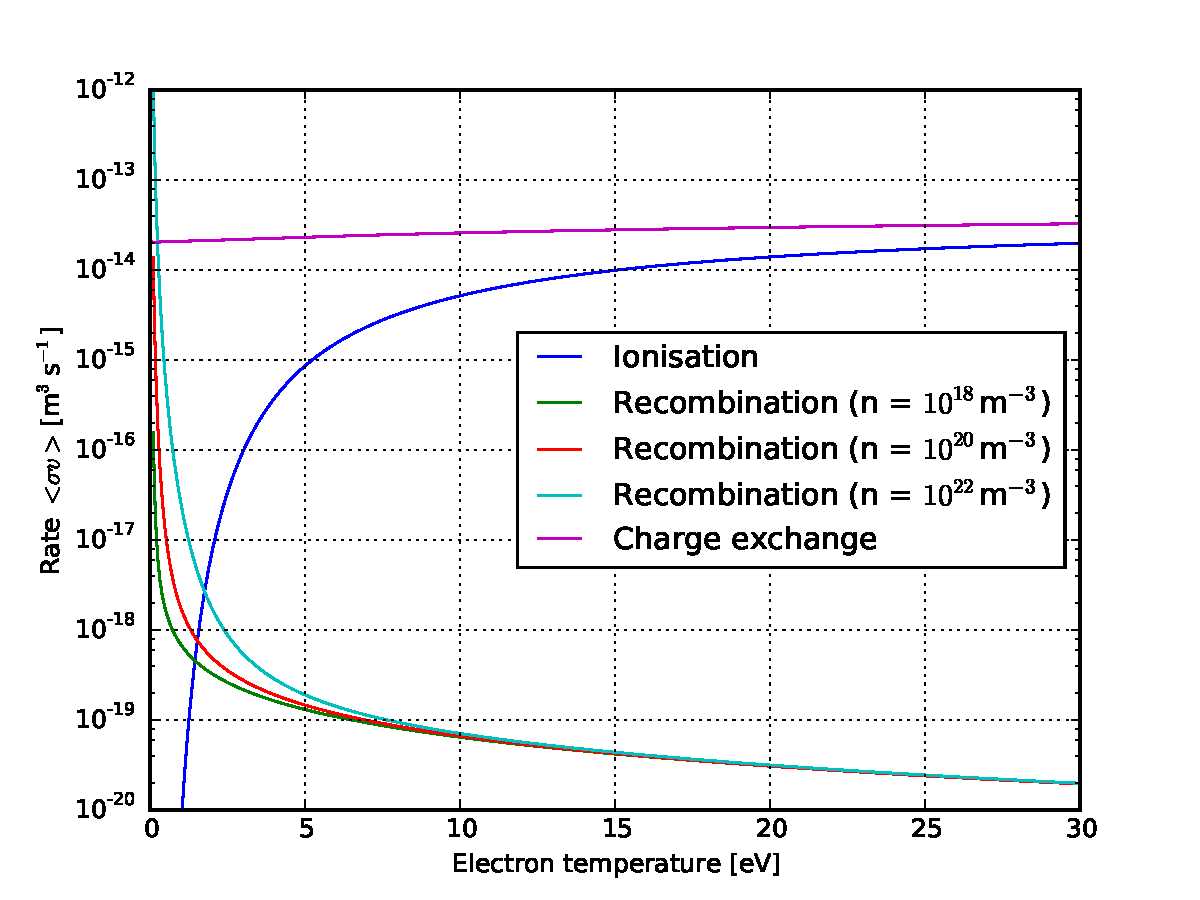
\includegraphics[width=0.7\columnwidth]{hydrogen.pdf}
\caption{Cross-sections [Thanks to E.Havlickova and H.Willett]}
\label{fig:sigma}
\end{figure}
Plots of these cross-sections are shown in figure~\ref{fig:sigma}. There are a few anomalies with this: charge exchange always has the highest cross-section of any process, and ionisation has a jump at $20$eV. The ionisation and
charge exchange rates do not depend on density, but recombination does so a typical range of values is shown.

\section{Heat conduction}
\label{sec:heatconduction}

Spitzer heat conduction is used
\begin{equation}
\kappa_{||e} = 3.2\frac{ne^2T\tau_e}{m_e} \simeq 3.1\times 10^4 \frac{T^{5/2}}{\ln \Lambda}
\end{equation}
which has units of W/m/eV so that in the formula $q = -\kappa_{||e} \nabla T$, $q$ has units of Watts per m$^2$ and $T$ has units of
$eV$. This uses the electron collision time:
\begin{equation}
\tau_e = \frac{6\sqrt{2}\pi^{3/2}\epsilon_0^2\sqrt{m_e}T_e^{3/2}}{\ln \Lambda e^{2.5} n} \simeq 3.44\times 10^{11} \frac{T_e^{3/2}}{\ln \Lambda n}
\end{equation}
in seconds, where $Te$ is in eV, and $n$ is in m$^{-3}$.

Normalising by the quantities in table~\ref{tab:normalisation} gives
\begin{equation}
\hat{\kappa}_{||e} = 3.2 \hat{n}\hat{T}_e\frac{m_i}{m_e}\tau_e\Omega_{ci}
\end{equation}
where hats indicate normalised (dimensionless) variables. 

\section{Non-uniform mesh}

An example of using a non-uniform grid is in \texttt{diffusion\_pn}.
The location $l$ along the field line as a function of normalised cell index $y$,
which goes from $0$ at the upstream boundary to $2\pi$ at the target, is
\begin{equation}
  l = L\left[ \left(2 - \delta y_{min}\right)\frac{y}{2\pi} -\left(1-\delta y_{min}\right)\left(\frac{y}{2\pi}\right)^2\right]
\label{eq:nonuniform_l}
\end{equation}
where $0<\delta y_{min}<1$ is a parameter which sets the size of the smallest grid cell, as a fraction
of the average grid cell size. The grid cell spacing $\delta y$ therefore varies as 
\begin{equation}
\delta y = \frac{L}{N_y} \left[ 1 + \left(1-\delta y_{min}\right)\left(1-\frac{y}{\pi}\right)\right]
\end{equation}
This is set in the BOUT.inp settings file, under the \texttt{mesh} section:
\begin{verbatim}
dy = (length / ny) * (1 + (1-dymin)*(1-y/pi))
\end{verbatim}
In order to specify the size of the source region, the normalised cell index $y$ at which
the location $l$ is a given fraction of the domain length must be calculated. This is done by
solving for $y$ in equation~\ref{eq:nonuniform_l}.
\begin{equation}
y_{xpt} = \pi\left[2 - \delta y_{min} - \sqrt{\left(2-\delta y_{min}\right)^2 - 4\left(1-\delta y_{min}\right) f_{source}}\right]/\left(1-\delta y_{min}\right)
\end{equation}
which is calculated in the BOUT.inp file as
\begin{verbatim}
y_xpt = pi * ( 2 - dymin - sqrt( (2-dymin)^2 - 4*(1-dymin)*source ) ) / (1 - dymin)
\end{verbatim}
where \texttt{source} is the fraction $f_{source}$ of the length over which the source is spread.
This is then used to calculate sources, given a total flux. For density:
\begin{verbatim}
source = (flux/(mesh:source*mesh:length))*h(mesh:y_xpt - y)
\end{verbatim}
which switches on the source for $y < y_{xpt}$ using a Heaviside function, then divides the flux
by the length of the source region $f_{source}L$ to get the volumetric sources.

\section{Numerical methods}

All variables are defined at the same location (collocated).
Several different numerical methods are implemented, to allow testing of their accuracy and robustness.

\subsection{Advection terms $\nabla\cdot\left(\mathbf{b}V_{||}f\right)$}

\subsubsection{Flux splitting, MinMod limiter}
\label{sec:fluxsplit}

The default method uses a combination of HLL-style flux splitting and MinMod slope limiting. 
Terms of the form $\nabla\cdot\left(\mathbf{b} f\right)$ are implemented as fluxes through cell boundaries:
\begin{equation}
\nabla\cdot\left(\mathbf{b} V f\right)_i \simeq \frac{1}{J\Delta y} \left[ F_{i+1/2} - F_{i-1/2}\right]
\end{equation}
where $F$ is the flux. This is calculated by linearly interpolating the velocity to the cell edges
\begin{equation}
V_{i+1/2} = \frac{1}{2}\left(V_{i} + V_{i+1}\right)
\end{equation}
The field being advected, $f$, is reconstructed from the cell centre values $f_i$ onto cell edges $f^L_i$ and
$f^R_i$:
\begin{equation}
f^L_i = f_i - \frac{1}{2}s \qquad f^R_i = f_i + \frac{1}{2}s
\end{equation}
where the slope $s$ is limited using the MinMod method:
\begin{equation}
s = \left\{\begin{array}{ll}
0 & \textrm{if $\operatorname{sign}(f_{i+1} - f_{i}) \neq \operatorname{sign}(f_{i} - f_{i-1})$} \\
f_{i+1} - f_{i} & \textrm{if $\left|f_{i+1} - f_{i}\right| < \left|f_{i} - f_{i-1}\right|$} \\
f_{i} - f_{i-1} & \textrm{otherwise}
\end{array}\right.
\end{equation}
In order to handle waves travelling both left and right, flux splitting handles characteristics moving left differently from characteristics moving right. 
In general this is problem dependent and computationally expensive, so here we adopt a simple approximation similar to an HLL splitting\footnote{A. Harten, P. D. Lax, and B. van Leer,''On Upstream Differencing and Godunov-Type Schemes for Hyperbolic Conservation Laws'', SIAM Review, 25(1), pp. 35-61, 1983}. 
We assume that the fastest waves in the system travel with speed $a$ (the sound speed) with respect to the flow, so that there are
waves travelling with $V+a$ and $V-a$. If the flow speed is supersonic then these waves are only in one direction, but for subsonic flows there is a flux in both directions. The fluxes between
cells are calculated using:
\begin{equation}
F_{i+1/2} = \left\{\begin{array}{ll}
f^R_iV_{i+1/2} & \textrm{if $V_{i+1/2} > a$} \\
f^L_{i+1}V_{i+1/2} & \textrm{if $V_{i+1/2} < -a$} \\
f^R_i\frac{1}{2}\left(V_{i+1/2} +a\right) + f^L_{i+1}\frac{1}{2}\left(V_{i+1/2} - a\right) & \textrm{otherwise}
\end{array}\right.
\label{eq:splitfluxes}
\end{equation}
Hence for subsonic flows the flux becomes $V_{i+1/2}\frac{1}{2}\left(f^R_i + f^L_{i+1}\right) + \frac{a}{2}\left(f^R_i - f^L_{i+1}\right)$, where the second term is a diffusion. When the solution is smooth, $f^R_{i}\simeq f^L_{i+1}$, the numerical method becomes central differencing and the diffusion goes to zero as $\Delta x^2$. Oscillatory solutions introduce dissipation, and the method becomes increasingly upwind as the flow becomes sonic.

\subsubsection{Nonlinear fluxes}
\label{sec:nonlinflux}

When advecting quantities which are a nonlinear combination of variables, such as $nV_{||}$, 
conservation properties can be slightly improved by using the following interpolation\footnote{F.N.Felten, T.S.Lund ``Kinetic energy conservation issues associated with the collocated mesh scheme for incompressible flow'' J.Comp.Phys. 215 (2006) 465-484}
\footnote{F.N.Felten, T.S.Lund ``Critical comparison of the collocated and staggered grid arrangements for incompressible turbulent flow'' Report ADP013663}
\footnote{Y.Morinishi et al. ``Fully Conservative Higher Order Finite Difference Schemes for Incompressible Flow'' J.Comp.Phys. 143 (1998) 90-124}:
\begin{equation}
\left(fg\right)^R = \frac{1}{2}\left(f^Rg^C + f^Cg^R\right)
\end{equation}
where superscript $C$ denotes cell centre, and $R$ right hand side. This method is implemented, using
MinMod interpolation for each variable.

\subsubsection{Central differencing}
\label{sec:central}

Central difference schemes have an advantage over upwind schemes, in that they do not need to take account
of wave speeds. The simple central differencing scheme produces large unphysical oscillations, due to the
decoupling of odd and even points in collocated schemes, but can (usually) be stabilised by adding dissipation. 
It is implemented here for comparison with other schemes.


\subsubsection{Skew symmetric central differencing}
\label{sec:skewform}

A simple modification to the central differencing scheme improves numerical stability, coupling nearby
points\footnote{S.Pirozzoli ``Stabilized non-dissipative approximations of Euler equations in generalized curvilinear coordinates'' J.Comp.Phys. 230 (2011) 2997-3014}
\footnote{A.E.Honein, P.Moin ``Higher entropy conservation and numerical stability of compressible turbulence simulations'' J.Comp.Phys. 201 (2004) 532-545}
The idea is to split the divergence terms into a ``skew-symmetric'' form
\begin{equation}
  \nabla\cdot\left(\mathbf{b} V_{||} f\right) = \frac{1}{2}\left[ \nabla\cdot\left(\mathbf{b} V_{||} f\right) + V_{||}\mathbf{b}\cdot\nabla f + f\nabla\cdot\left(\mathbf{b} V_{||}\right)\right]
\end{equation}
Each of the terms on the right are then discretised with standard 2nd-order central differences.
This method can avoid the need for additional dissipation, or be stabilised with a smaller viscosity than
the simple central differencing method.

\subsection{Artificial viscosity}
\label{sec:viscos}

Artificial viscosity (\texttt{viscos} input) is implemented as a diffusion of momentum in index space, so that the diffusion coefficient varies as $\Delta y^2$.
\begin{equation}
  \frac{\partial}{\partial t}\left(nV_{||}\right)_i = \ldots + \nu\left[ \left(V_{i+1} - V_i\right)J_{i+1/2} - \left(V_i - V_{i-1}\right)J_{i-1/2} \right]/J_i
\end{equation}
where $J$ is the Jacobian, subscript $i$ indicates cell index, and $J_{i+1/2} = \left(J_i + J_{i+1}\right)/2$.


\end{document}
